\documentclass[]{article}
\setlength{\evensidemargin}{-0.25in}
\setlength{\oddsidemargin} {-0.25in}
\setlength{\textwidth}     {+7.00in}

\setlength{\textheight}    {+8.50in}
\usepackage{graphicx}
\usepackage{hyperref}
\graphicspath{ {./images/}}

%opening
\title{Denver Property Analysis}
\author{Nicholas Stevenson, Sydney John, Tri Le}
\date{May 4, 2022}

\begin{document}

\maketitle
\section{The Data}
We examined the Denver real estate prices of commercial and residential property types starting in 2004 until present day, using the data to draw conclusions on the growth and value of real estate specific for each neighborhood in the city.
\subsection{Interesting Aspects of the Data}
\subsection{Obtaining the Data}
The data was obtained from Denver's open Data Catalog. It has an open data license, so we have no legal restrictions on use of the data. A link is provided here: \href{https://www.denvergov.org/opendata/dataset/city-and-county-of-denver-real-property-sales-and-transfers}{LINK}
\section{Table Information}
We have three tables created from our loaded data. The data was obtained from a single data set, then separated by a python script to be easier and faster to work with.

\subsection{Property}
The property table contains information pertaining properties that were involved in the transactions. Attributes include the transaction number, sale price, grantor, grantee, class, mkt$\_$clus, d class number, and neighborhood number. The table will have foreign keys of d class and neighborhood numbers to join them with the d class and neighborhood tables respectively.

\begin{table}[h!]
	\begin{center}
		\caption{Property}
		\label{tab:table1}
		\begin{tabular}{c|c|c|c|c|c|c|c|c} 
			\textbf{transaction} & \textbf{reception date} & \textbf{sale price} & \textbf{grantor} & \textbf {grantee} & \textbf{class} & \textbf{mkt clus} & \textbf{d class} & \textbf{nbhd 1} \\
			\hline
			4 & 20150121 & 9350000 & PEP & MENIFEE  & C & & 223 & 4 \\
			120 & 20170721 & 12500000 & LNR & ACM & A & 3 & 214 & 4\\
			141 & 20200313 & 9000000 & ACM & LYON & H & 52 & 193 & 4\\
		\end{tabular}
	\end{center}
\end{table}


\subsection{Neighborhood}
The neighborhood table contains identification information of the neighborhoods that the properties reside in.  The data consists of only two attributes; an id column and a name column. The property table references this table using a foreign key to the neighborhood id. Example lines of the table are shown below in Table 2.
 
 
 \begin{table}[h!]
 	\begin{center}
 		\caption{Neighborhood}
 		\label{tab:table2}
 		\begin{tabular}{c|c}
 			\textbf{number} & \textbf{name}\\
 			\hline
 			1 & MONTEBELLO\\
 			2 & PARKFIELD\\
 			3 & GREEN VALLEY\\
 		\end{tabular}
 	\end{center}
 \end{table}

\subsection{D$\_$Class} 
The d$\_$class table contains the d$\_$class$\_$id, labeled by id, and the english representation, labeled by name. We use the name of the d$\_$class to determine if the property is residential or commercial. The property table references this table using a foreign key on the id. Examples lines from the table are shown in Table 3.

\begin{table}[h!]
	\begin{center}
		\caption{D Class}
		\label{tab:table3}
		\begin{tabular}{l|c} % <-- Alignments: 1st column left, 2nd middle and 3rd right, with vertical lines in between
			\textbf{id} & \textbf{name}\\
			\hline
			070 & DRY FARM LAND\\
			214 & RESIDENTIAL - MULTI UNIT APTS \\
			222 & COMMERCIAL - HOTEL\\
		\end{tabular}
	\end{center}
\end{table}

\subsection{ERD Diagram}
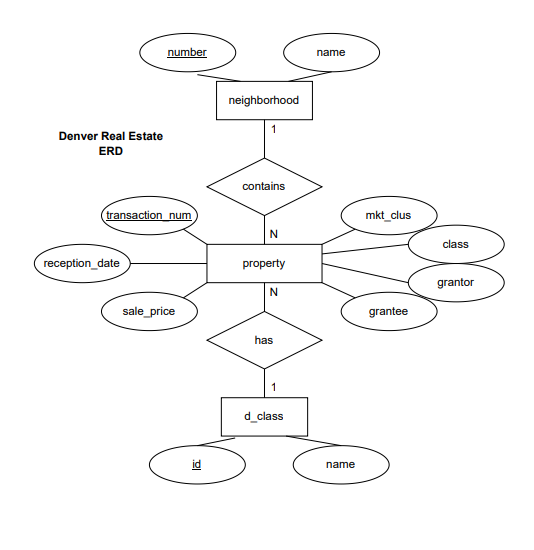
\includegraphics{ERD}

\section{Data Processing}
\subsection{Cleaning the Data}
We used a combination of python scripts and visual inspection to clean our csv formatted data set. First we inspected the raw data within excel and determined what columns and relationships we wanted to transfer into our database. After identifying the columns and the relationships we used a python script to create derivative csv files characterized by the columns and their relationships, essentially creating one csv file for each entity we have in our ERD. Then we used the ERRORS from the copy command to fix any ill formatted data within our dataset. 

\subsection{Loading the Data}
We used a combination of python scripts and visual inspection to clean our csv formatted dataset. First we inspected the raw data within excel and determined what columns and relationships we wanted to transfer into our database. After identifying the columns and the relationships we used a python script to create derivative csv files characterized by the columns and their relationships, essentially creating one csv file for each entity we have in our ERD. The python script is provided in the zip file. Then we used the ERRORS from the copy command to fix any ill formatted data within our dataset. 

\section{Analyzing the Data}

\end{document}
